\documentclass{beamer}
%
% Choose how your presentation looks.
%
% For more themes, color themes and font themes, see:
% http://deic.uab.es/~iblanes/beamer_gallery/index_by_theme.html
%
\mode<presentation>
{
  \usetheme{default}      % or try Darmstadt, Madrid, Warsaw, ...
  \usecolortheme{default} % or try albatross, beaver, crane, ...
  \usefonttheme{serif}  % or try serif, structurebold, ...
  \setbeamertemplate{navigation symbols}{}
  \setbeamertemplate{caption}[numbered]
} 

\usepackage[english]{babel}
\usepackage[utf8x]{inputenc}
\usepackage[font=scriptsize,labelfont=bf]{caption}

\title[APC 524 Design Review]{Tabulation of Chemical Source Terms for Turbulent Combustion Simulations}
\author{Emmet Cleary \\
Daniel Floryan \\
Jeffry Lew \\
Bruce Perry \\
Emre Turkoz} 
\date{December 2, 2014}

\begin{document}

\begin{frame}
  \titlepage
\end{frame}

% Uncomment these lines for an automatically generated outline.
%\begin{frame}{Outline}
%  \tableofcontents
%\end{frame}

\section{Introduction}
\begin{frame}{Introduction}
\begin{figure}
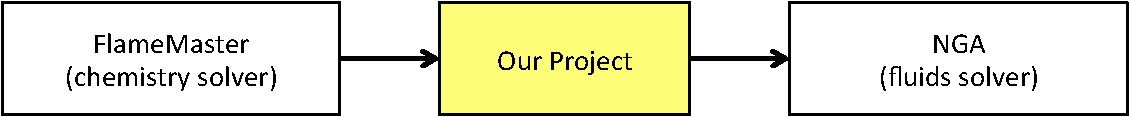
\includegraphics[width=\textwidth]{scope.pdf}
\end{figure}
\vskip 5mm
Key Capabilities:
\begin{itemize}
\item Sorting
\item Monotonicity checking
\item Convolution
\item Interpolation
\end{itemize}
\vspace{12pt}
SWIG will be used to interface C++ and Python.

\end{frame}

\section{Flowcharts}

\subsection{Progress Variable}
\begin{frame}{Progress Variable}
\begin{figure}
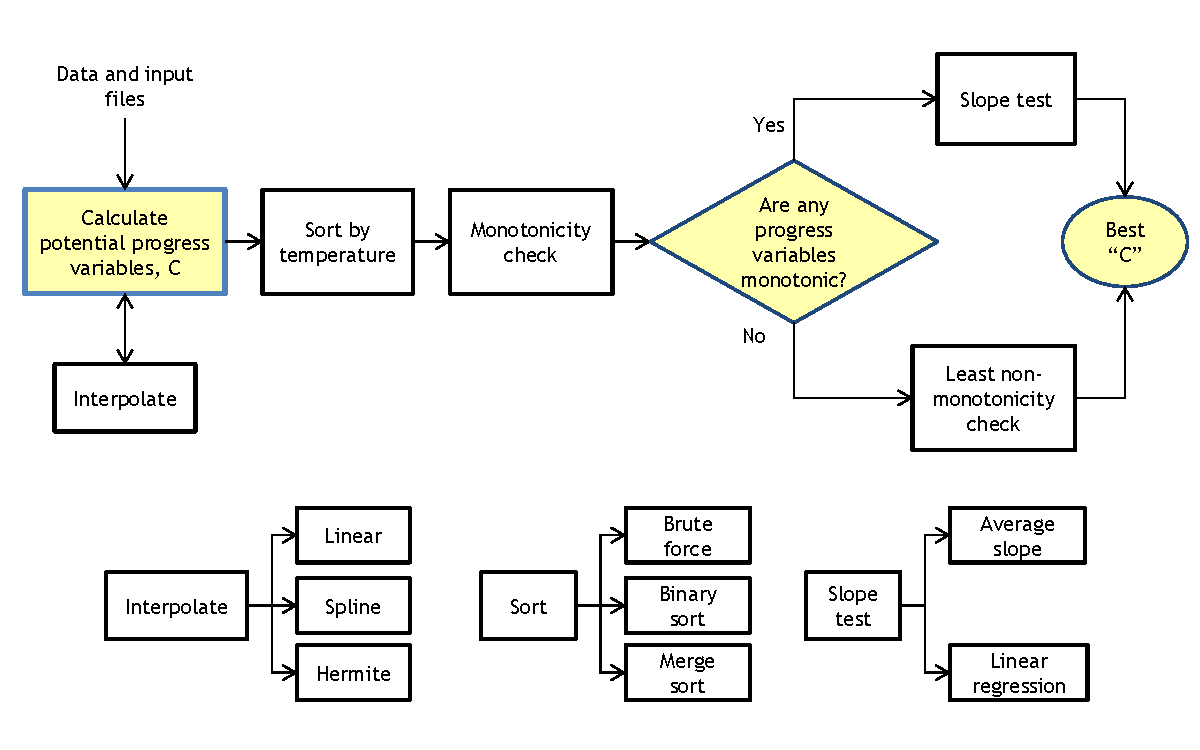
\includegraphics[width=\textwidth]{diagram_1_shortened_v1.pdf}
\end{figure}
\end{frame}

\subsection{Table Generation}
\begin{frame}{Table Generation}
\begin{figure}
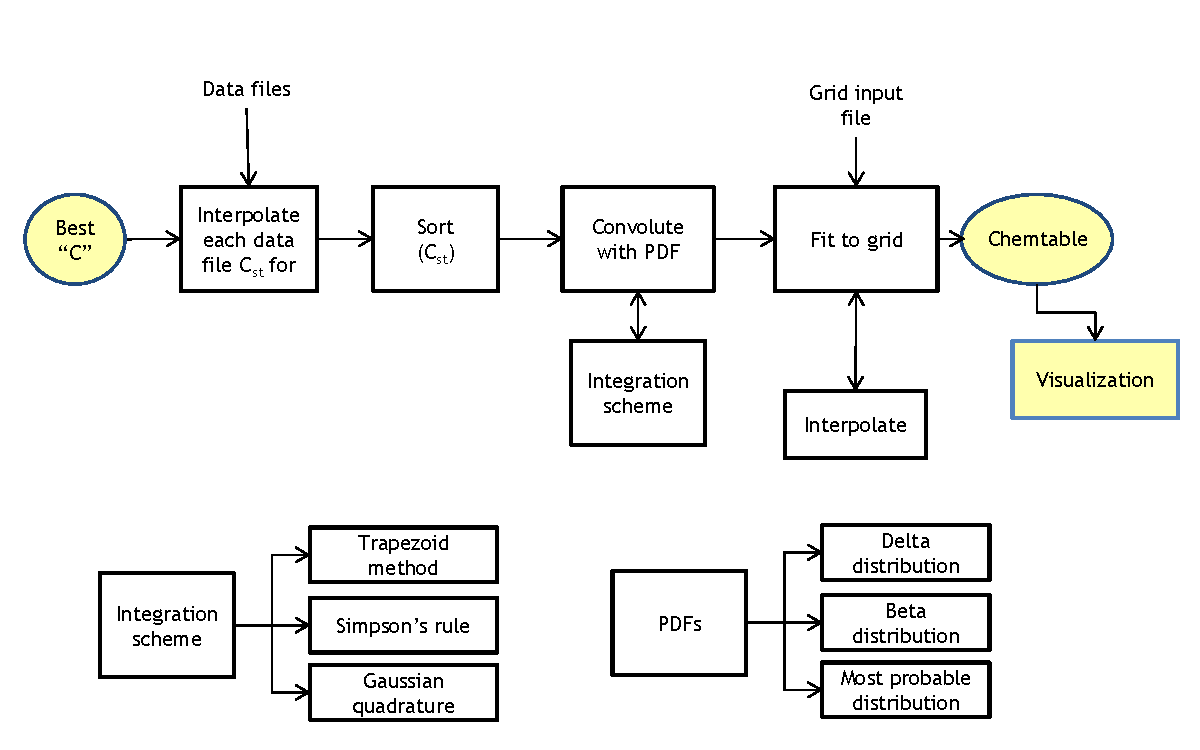
\includegraphics[width=\textwidth]{diagram_2_shortened_v1.pdf}
\end{figure}
\end{frame}

\end{document}
